\chapter{Hidden Markov Model}\label{ch:hmm-chords}
Identifichiamo la sequenza di note della melodia con Y e l'armonizzazione sottostante con C, in particolare $y_t$ rappresenta la nota della melodia al tempo t e $c_t$ rappresenta lo stato armonico al tempo t. \\
E' stato utilizzato un modello di Markov con assunzioni del primo ordine, ovvero tale per cui vale:
\begin{equation}
P(c_t|c_{t-1},...,c_0) = P(c_t|c_{t-1})
\end{equation}
\begin{equation}
P(y_t|c_t,...,c_0,y_{t-1},...,y_0) = P(y_t|c_t)
\end{equation}
In particolare vengono costruiti due modelli di Markov, uno relativo ai corali in tonalità maggiore ed uno relativo ai corali in tonalità minore.
Il dataset iniziale è stato così suddiviso:
\begin{itemize}
\item 121 file di training (tonalità maggiore)
\item 81 file di test (tonalità maggiore)
\item 108 file di training (tonalità minore)
\item 72 file di test (tonalità minore)
\end{itemize}
\section{Training}
Il modello di Markov è stato costruito utilizzando la libreria Python "hmmlearn". \\
Avendo a disposizione sia gli stati visibili che gli stati nascosti non è stato necessario apprendere i parametri del modello tramite Expected Maximization, ma sono state invece costruite, utilizzando i dati, sia la matrice di transizione che la matrice di emissione.\\
In particolare per gestire il grande numero di zero all'interno di queste matrici si è proceduto applicando uno smoothing additivo sommando 0.01 ad ogni elemento delle matrici prima di normalizzarle per renderle stocastiche.
Anche la distribuzione iniziale di probabilità è stata calcolata utilizzando i dati, andando a dare una probabilità maggiore agli stati più frequenti all'inizio dei corali. \\
Il modello relativo alla tonalità maggiore (chords-dur) contiene 2815 stati nascosti e 55 stati visibili, mentre il modello relativo alla tonalità minore (chords-moll) contiene 2593 stati nascosti e 52 stati visibili.
\section{Testing}
Per ogni file di test viene generata, data la relativa sequenza di stati visibili, la sequenza più probabile di stati nascosti utilizzando l'algoritmo di Viterbi.
In tabella viene mostrato quanto gli stati nascosti prodotti siano equivalenti a quelli reali. \\
INSERIRE TABELLA RISULTATI
Come ci si aspetta i risultati sono abbastanza diversi in quanto il modello non ha alcuna informazione relativa ad esempio al periodo in cui è stato composto un determinato corale, oppure per quale occasione. Senza l'ausilio di ulteriori dati esterni sarebbe impossibile ricostruire perfettamente i corali originali.
\begin{figure}[H]
	\centering
	\caption{A sx l'originale, a dx l'armonizzazione più probabile del nostro modello}
	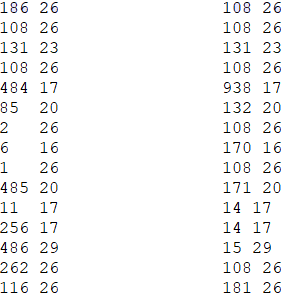
\includegraphics{figures/viterbi.png}
	\label{viterbi}
\end{figure}
\noindent
Interpretare i risultati non è semplice, la figura \ref{viterbi} non è per nulla esplicativa, se ragionassimo in termini di accuratezza sembrerebbe che il nostro modello sia assolutamente pessimo, ma l'obiettivo non è quello di costruire risultati identici all'originale, ma armonizzazioni musicalmente accettabili e orecchiabili. \\
Presentare i risultati sotto forma di spartito musicale può favorirne la comprensione per chi è in grado di leggerli, ma non è abbastanza per chi non ha una approfondita conoscenza del dominio. Per questo motivo è necessario trasformare i risultati ottenuti in un formato musicale udibile.
\section{Sampling}
E' possibile anche generare sequenze di stati in accordo alla distribuzione di probabilità del modello. Consideriamo $\alpha_{t-1}(j)$, la probabilità di avere visto le prime $t - 1$ osservazioni di una sequenza ed essere finiti nello stato j, possiamo calcolare la probabilità di aver visto i primi $t - 1$ eventi, essere finiti in uno stato qualsiasi, e poi eseguire una transizione verso uno stato k:
\begin{equation}
P(y_0 = Y_{i0}, y_1 = Y_{i1}, ...,y_{t-1}=Y_i_{t-1})
\end{equation}
\section{Ricostruzione dei risultati}
Mediante l'utilizzo dello script "hmm-output-expand.py" è possibile ricostruire, a partire dalle coppie [hidden-visible] costruite da Viterbi, il file in notazione musicale.\\
In questo punto notiamo uno dei principali problemi del modello costruito, ovvero la mancanza di informazione temporale relativa agli stati visibili e nascosti. \\
Per ricostruire il file musicale è necessario rispettare le cadenze della musica originale e ciò rende molto complicato ad esempio generare nuova musica con il modello. Questo banalmente perchè la musica generata, per quanto orecchiabile, non avrà una struttura temporale sensata ed ogni nota avrà la stessa lunghezza, come tale la melodia prodotta risulterà molto più "robotica" e poco reale.
\section{Generazione del file MIDI}
Il protocollo MIDI è uno standard per la composizione e riproduzione di file musicali. Tramite lo script "chorale2midi.py" è possibile convertire i file testuali generati nel passaggio precedente in formato MIDI in modo tale da poterli riprodurre. \\
\section{Armonizzazione di musica moderna}
Il modello di Markov proposto è teoricamente in grado di armonizzare una melodia qualsiasi, dato un file MIDI è possibile estrarre le note della melodia e utilizzarle come base per l'armonizzazione. Il task è però particolarmente complicato perchè la struttura dei file di input è molto rigida, in particolare:
\begin{itemize}
\item la durata delle note, nel file MIDI, deve necessariamente essere multiplo della durata di una nota semiminima (1/4)
\item in una battuta ci possono essere massimo quattro note
\item non c'è mai una pausa tra note nella stessa battuta
\end{itemize} 
Il primo motivo è facilmente gestibile andando ad arrotondare la durata delle note al multiplo di 240 più vicino, ciò altera leggermente la melodia, ma non abbastanza da rovinarla.\\
Il secondo è un problema legato principalmente a canzoni veloci o complesse che non sono gestibili dal modello. \\
L'ultimo problema è quello forse più complicato da gestire, in quanto richiede l'aggiunta di note fittizie all'interno del file che verranno poi trattate come delle pause.\\
In Python non sono presenti librerie in grado di gestire facilmente file MIDI in ingresso, per questo motivo la musica moderna è stata trascritta manualmente nei file di ingresso, per mancanza di tempo non è stato possibile effettuare automaticamente questo compito.
A questo si aggiunge il fatto che, molto spesso, i file MIDI non sono correttamente divisi per canali (idealmente uno strumento per canale) e ciò rende ancora più complicato il parsing automatico di questi file.\\
A puro scopo dimostrativo e ludico abbiamo provato ad armonizzare varie melodie moderne per vedere come suonerebbero se fossero state composte da Bach sotto forma di corale.